%-----------------------------------------------------------------------------------------
\clearpage
\section{Project Plan and Time Management}
%-----------------------------------------------------------------------------------------

 

\subsection{Development Approach}

Traditionally, Waterfall Model is used as the guiding methodology for many projects. It uses linear flow to show the progress of the project and allow people to understand easily the further steps after completing the previous step. It is suitable for sequential design, which means it may be impossible for developers to back to steps if they found some problems at last. 
The progress of the Waterfall Model is, according to\cite{Adenowo2013}, include 5 phases: Requirement analysis, design, implementation, testing, and operation and maintenance.(See Figure \ref{waterfall})

\begin{figure}[h]
	\centering	
	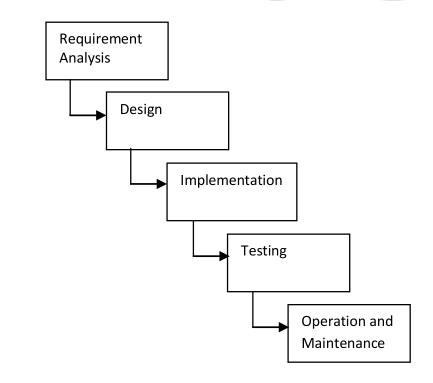
\includegraphics[width=6cm, height=6cm]{Figs/Waterfall-Model}\\[1ex]
	\caption{The 5 phases of Waterfall Model ( \cite{Adenowo2013})}
	\label{fig:waterfall}
\end{figure}

However, when projects run out of time, testing phase will be cut, which may lead to poor quality of the outcomes. In addition, the operation is in the last step, developers may be unaware of where they’ve gone and what they’ve done, it is invisible for developers to know the progress. Last but not least, it is impossible for developers to change until the last phase.

\begin{figure}[h]
	\centering	
	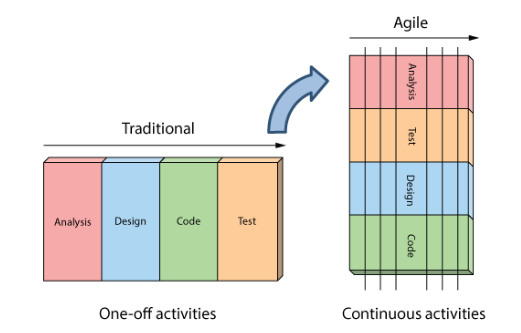
\includegraphics[width=6cm, height=6cm]{Figs/Waterfull-Agile}\\[1ex]
	\caption{Comparison between Waterfall methodology and Agile methodology (\cite{Agile vs Waterfall})}
	\label{fig:waterfallAgile}
\end{figure}

Unlike with the Waterfall methodology which separates the whole project into several phases and implement it step by step, the Agile methodology separates the project into several tasks and every task is implemented in several phases. By doing this, it is changeable for developers when they find mistakes. And hence the quality and visibility issues of Waterfall methodology are solved. Hence, we adopt Agile as our guiding methodology when implementing this project.

\subsection{Project Timetable}

This section indicates time management for the project. These project separates into 5 phases \cite{Laramee} as follow:

\begin{itemize}
	\item \textbf{1. }Requirements Specification; 
	Data Preprocessing; 
	Project Presentation;
	Exploring existing tools; 
	Project Specification; 
	 complicated data processing techniques.
	\item \textbf{2. }Software Design;
	Candidate Classes and Responsibilities;
	Candidate Hierarchy;
	Collaboration and Subsystems;
	\item \textbf{3. }Implementation;
	Software Development;
	GUI;
	\item \textbf{4. }Debugging and Testing;
	\item \textbf{5. }Documentation;
\end{itemize}

Figure \label{gantterChart} indicates the Gantt of the project timeline. This project initiated from 17th February, and the final deadline is 30th September. In every phase, there are several tasks to be done. Most of the tasks in phase one has been done, except data preprocessing which needs more time to process more text data. The second phase is expected to finish before July. So more can be used in the implementation phase. Software implementation is supposed to spend the most time, which will be executed according to the designs done by previous work. After the implementation, simple GUI framework will be done. From the middle of August, the project is expected to start debugging and testing phase. Finally, a report and Doxygen will be done in September. 

\begin{figure}[h]
	\centering	
	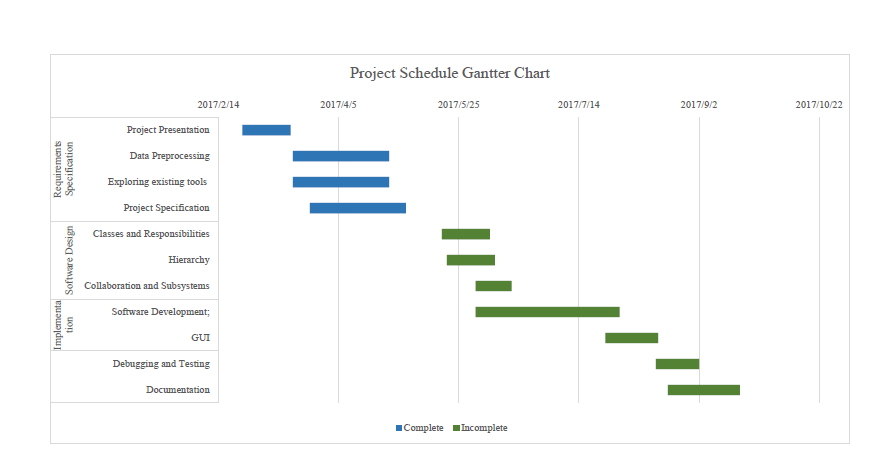
\includegraphics[width=6cm, height=6cm]{Figs/Gantter-Chart}\\[1ex]
	\caption{Gantt chart for project timeline }
	\label{fig:gantterChart}
\end{figure}


\subsection{Risk Analysis}

This part is about the potential risks which may happen when doing this project.

Figure \label{riskAnalysis} mapping the analysis of these risks:\.
The first risk is that the author may lack of the knowledge when carrying out the project. The probability is medium as the limited time author has been studying the computer science. The impact has been considered as high because the project will progress slowly and face obstacles without support of essential knowledge. So, the regular meeting with the supervisor is important to consult the difficulties encountered during the process.   
The second risk is that the whole project may be finished after the deadline. The possibility is considered medium due to the possibility of other risks. Lack of essential knowledge, problems in programming, or lack of project management skills may lead to the delay. The author should apply for delaying submission if this will happen in advance. 
The third risk identified is personal illness of the author. It is a low possibility risk with medium impact for the project. To deal with this case, keeping a good healthy is important to author herself. In addition, there is welfare service department on campus and the author has the international student’s insurance. 
Equipment failure is identified as the fourth risk. It is classified as medium in terms of both possibility and impacts. Yet there are computer equipments on campus and the library open 24 hours so that the resources of university are available every day. 
Data loss is considered as the fifth risk. the possibility of this happening is low but will cause high impact to the project. To avoid this situation, using the application Github for regular backup is necessary. 
The last risk is lacking project management skills to implement the project. This is considered as medium possibility to happen with high impacts to the project. In this case, a strict plan following rules of Agile software development methodology is important.

\begin{figure}[h]
	\centering	
	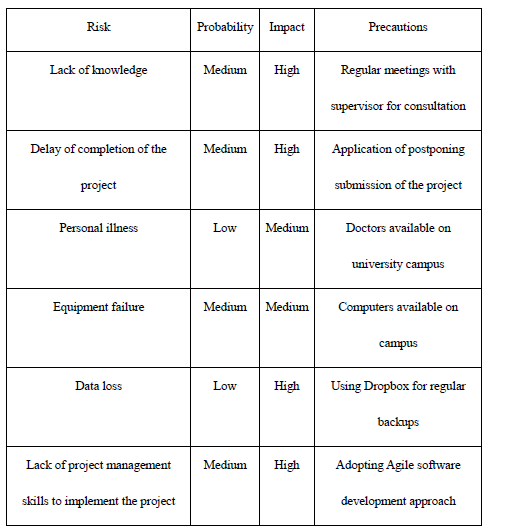
\includegraphics[width=6cm, height=6cm]{Figs/Risk-Analysis}\\[1ex]
	\caption{Risk Analysis Table }
	\label{fig:riskAnalysis}
\end{figure}

